%% It is just an empty TeX file.
%% Write your code here.
\chapter{Attached files}
Together with this thesis, an electronic version is attached containing supplementary results of the work done. The results presented in this thesis are just illustrative and require deeper studying for better understanding. Attached figures, source codes and scripts may serve as help in generating own test patterns and evaluating existing results. The sections are named after the folder structure.
\section{VHDL}
In order to get started, an environment needs to be set up. The attached VHDL codes allow to build a testing system within short time. The $DDENCODER.vhd$ is an isolated Encoder, also available in version with error injection interface. The $DDECODER.vhd$ is an isolated Decoder. The Test Bench consists of a top module residing in $Engine.vhd$ and submodules for address generation in $addr.vhd$ and internal Test Engine in $shift.vhd$. Additional module is the configuration unit, which is a custom AXI IP. $Myip\_AXI\_Interconnect\_v1\_0.vhd$ is a top module containing Freq\_Monitor and an internal AXI module. The example shows how to build the Test Bench using a ZedBoard.
To build the test environment, the instantiation of the Zynq processing unit with 2 BRAMS is required. The BRAMS are configured as True Dual Port BRAMS. Only one port of each memory is connected to the BRAM Controller, while the other is connected to the Test Engine, one to the input, one to the output. Together with all corresponding pins - the address and write enable signal. The clock Wizard is set to MMCM mode with Dynamic Reconfiguration and two output clocks. The clk\_out1 is connected to clk\_var of the Test Engine, while clk\_out2 to the clk\_mem. Both clocks also need to be connected to the AXI\_CFG unit. The Configuration Unit feeds the Test Engine with initial and maximal addresses, enable pin and reset pin. The ready pin needs to be connected with the corresponding pin in the Test Engine.
The Test Engine default configuration remains unchanged, only the UUT\_width needs to be adjusted to the width of the UUT interface. The UUT\_clk, UUT\_dout and UUT\_din are to be connected to tested design.

\section{GUI}

The GUI Folder contains the User Interface Program. In this program  XML Files for test are chosen and test parameters set. The interface is showed in \autoref{fig:GUI}. 

\begin{figure}[h]
\centering
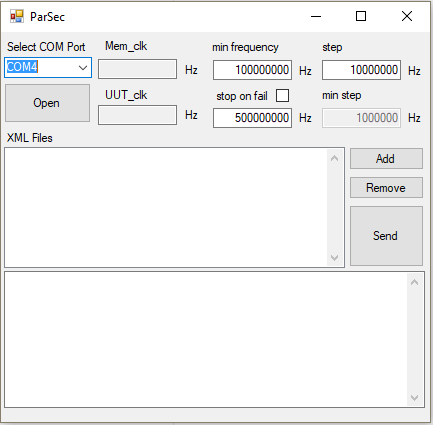
\includegraphics[width=.5\textwidth]{figures/GUI.PNG}
\caption{The User Interface}
\label{fig:GUI}
\end{figure}

Firstly a COM port, to which the board is connected, needs to be opened. Then the XML files chosen. Multiple selection is possible. If the XML file is configured to have no test frequency, the values from the interface are used. The initial frequency, the stop frequency and the step need to be adjusted. If the field "stop on fail" is marked, the test will run with initial step, until first test fails and then lower the step and run again. The procedure repeats, until the minimum step is achieved. During the test, information about the progress is displayed in the bottom text box.

The folder contains also three files with precomputed frequency setups. They are used for setting the parameters of the MMCM logic in the FPGA and stored as look-up tables, to spare time.

\section{SDK}
This folder contains two projects that need to be placed in the SDK environment. The TestEngine Project is the main project. 

\section{Tests}
In this group of folders, the generated $xml$ files reside together with MATLAB (version 2015b) scripts, to generate new files and to evaluate old ones. THe REsults folder contains test results in compressed files. Every archive contains a $html$, $xml$ and $mat$ file. They all represent the same data, but in different form. The $html$ file is destined to view the raw data in a fast graphical form. The $xml$ file can be used to import the data into some other environment. The $mat$ file contains a structure, representing the $xml$ file contents in MATLAB format. The evaluating scripts allow to choose the input format to be either $xml$ or $mat$, while the $mat$ file is always saved after processing the $xml$ file to save time in the future. It may be recommended to keep the files smaller, by dividing the test into more files, because the processing is memory intensive and not optimal for bigger file sizes.
Each script contains instructions to generate figures visible in this thesis. The data file names are descriptive, so listing them is not necessary. All parameters that can be changed in scripts are placed at the beginning. It may be however needed to edit or uncomment certain parts to achieve desired results. The scripts should rather act as help in creating own test patterns and result analyzers. All details according pattern generation have been documented in this thesis before.

The electronic version contains also an archive of the project in \LaTeX 
